\documentclass[b5paper,oneside,british,intoc,bibliograph=totoc,index=totoc,BCOR10mm,twoside,openright]{book}
\usepackage[LGR,T1]{fontenc}
%\usepackage[utf8]{inputenc}
\usepackage{inputenc}
\usepackage{fancyhdr}
\pagestyle{fancy}
\setcounter{tocdepth}{3}
\usepackage{babel}
\usepackage{float}
\usepackage{textcomp}
\usepackage{amsmath}
\usepackage{amsthm}
\usepackage{graphicx}
\usepackage{setspace}
\usepackage{subcaption}
\usepackage{csquotes}
\usepackage{pdflscape}
\usepackage{graphicx}
\usepackage[toc,page]{appendix}
\usepackage{algorithm}
\usepackage{algpseudocode}


\setstretch{1.2}
\usepackage[unicode=true,pdfusetitle,
 bookmarks=true,bookmarksnumbered=false,bookmarksopen=false,
 breaklinks=false,pdfborder={0 0 1},backref=false,colorlinks=false]
 {hyperref}
\hypersetup{
 pdfpagelayout=OneColumn, pdfnewwindow=true, pdfstartview=XYZ, plainpages=false}

\makeatletter
\g@addto@macro{\UrlBreaks}{\UrlOrds}


\newcommand*\LyXThinSpace{\,\hspace{0pt}}
\pdfpageheight\paperheight
\pdfpagewidth\paperwidth

\DeclareRobustCommand{\greektext}{%
  \fontencoding{LGR}\selectfont\def\encodingdefault{LGR}}
\DeclareRobustCommand{\textgreek}[1]{\leavevmode{\greektext #1}}
\ProvideTextCommand{\~}{LGR}[1]{\char126#1}

\providecommand{\tabularnewline}{\\}
%% A simple dot to overcome graphicx limitations
\newcommand{\lyxdot}{.}

\numberwithin{equation}{section}
\numberwithin{figure}{section}

\usepackage{amsthm,amsmath}
%\RequirePackage{hyperref}
\usepackage{graphicx}
\usepackage{rotating}
\usepackage{colortbl}
\usepackage{url}
\usepackage{siunitx}
\usepackage{algorithm}
\usepackage{algpseudocode}


\usepackage[a4,cam,center]{crop}

\usepackage{multicol}
\usepackage{listings}
\usepackage{xcolor}
\definecolor{hellgelb}{rgb}{1,1,0.9}
\definecolor{colKeys}{rgb}{0,0,1}
\definecolor{colIdentifier}{rgb}{0,0,0}
\definecolor{colComments}{rgb}{1,0,0}
\definecolor{colString}{rgb}{0,0.5,0}
\lstset{%
float=hbp,%
identifierstyle=\color{colIdentifier}, %
keywordstyle=\color{colKeys}, %
stringstyle=\color{colString}, %
commentstyle=\color{colComments}, %
columns=flexible, %
tabsize=2, %
frame=single, %
extendedchars=true, %
showspaces=false, %
showstringspaces=false, %
numbers=left, %
numberstyle={\tiny\ttfamily}, %
stepnumber=5, %
breaklines=true, %
backgroundcolor=\color{hellgelb}, %
breakautoindent=true, %
basicstyle={\small\ttfamily},%
language=C,%
captionpos=b%
}


\usepackage{fancyheadings}
\pagestyle{fancy}
\renewcommand{\chaptermark}[1]%
{\markboth{\uppercase{\thechapter.\ #1}}{}}
\renewcommand{\sectionmark}[1]%
{\markright{\uppercase{\thesection.\ #1}}}

\newcommand{\helv}{%
\fontfamily{phv}\fontseries{b}\fontsize{9}{11}\selectfont}
\lhead[\helv \thepage]{\helv \rightmark}
\rhead[\helv \leftmark]{\helv \thepage}
\cfoot{}

% non voglio sottosezioni e paragrafi nella table of content
\renewcommand\l@paragraph[2]{}
\renewcommand\l@subsubsection[2]{}

\usepackage[backend=bibtex8,style=nature]{biblatex}
\addbibresource{bibs/PhDThesisBib.bib}
\DeclareSymbolFont{extraup}{U}{zavm}{m}{n}
\DeclareMathSymbol{\varheart}{\mathalpha}{extraup}{86}


% limits underneath
\DeclareMathOperator*{\argminA}{arg\,min} % Jan Hlavacek
\DeclareMathOperator*{\argminB}{argmin}   % Jan Hlavacek
\DeclareMathOperator*{\argminC}{\arg\min}   % rbp

\newcommand{\argminD}{\arg\!\min} % AlfC

\newcommand{\argminE}{\mathop{\mathrm{argmin}}}          % ASdeL
\newcommand{\argminF}{\mathop{\mathrm{argmin}}\limits}   % ASdeL

% limits on side
\DeclareMathOperator{\argminG}{arg\,min} % Jan Hlavacek
\DeclareMathOperator{\argminH}{argmin}   % Jan Hlavacek
\newcommand{\argminI}{\mathop{\mathrm{argmin}}\nolimits} % ASdeL

\newcommand{\cs}[1]{\texttt{\symbol{`\\}#1}}

%%%%%%%%%%%%%%%%%%%%%%%%%%%%%%%%%%%%%%%%%%y

\usepackage[Lenny]{fncychap/fncychap}
\setcounter{tocdepth}{6}

\makeatother

\usepackage{listings}
\lstset{breaklines=true,
fontadjust=true,
frame=lines,
language=R,
tabsize=2}

%\startlocaldefs
\algnewcommand\algorithmicinput{\textbf{INPUT:}}
\algnewcommand\INPUT{\item[\algorithmicinput]}
\algnewcommand\algorithmicoutput{\textbf{OUTPUT:}}
\algnewcommand\OUTPUT{\item[\algorithmicoutput]}
%\endlocaldefs


\begin{document}
\pagestyle{empty}

\begin{center}
UNIVERSIT\'A DEGLI STUDI DI SALERNO
\par\end{center}

\begin{center}
DOTTORATO IN MANAGEMENT \& INFORMATION TECHNOLOGY
\par\end{center}

\bigskip{}

\begin{center}
\includegraphics[scale=0.2]{img/logoUnisa}
\par\end{center}

\bigskip{}

\begin{center}
CURRICULUM: INFORMATION SECURITY \& INNOVATION SYSTEMS
\par\end{center}

\begin{center}
COORDINATORE: Ch.mo. Prof. Antonelli Valerio
\par\end{center}

\begin{center}
Ciclo XVII N.S.
\par\end{center}

\vspace{1.5cm}

\begin{center}
Novel tools for reproducible 

Next Generation Sequencing data analysis and integration 
\par\end{center}

\vspace{1.5cm}

\textbf{\large{}Relatori}\hfill{}\textbf{\large{}Candidato}{\large \par}

Ch.mo. Prof. Tagliaferri Roberto\hfill{}Righelli Dario

Ch.mo. Prof. Angelini Claudia\hfill{}Matr. 8800800010

\vspace{1.5cm}

\begin{center}
ANNO ACCADEMICO 2017/2018
\par\end{center}

\cleardoublepage

\begin{quotation}
\begin{flushright}
\textit{
How to reach a goal? \\
Without haste but without rest\\
Goethe}
\par\end{flushright}
\end{quotation}


\cleardoublepage
% \phantomsection
\addcontentsline{toc}{chapter}{Acknowledgements}

Add acknowledgements here
%\include{acknowledgements}

\cleardoublepage

\addcontentsline{toc}{chapter}{Abstract}

Write your abstract here
\section*{Abstract}
{\setlength{\parindent}{0cm}
Massive parallel sequencing technologies are producing a vast amount of genome-wide data about cells, tissues and model organisms, useful to understand many of biological mechanisms, like protein-chromatin interactions (e.g. ChIP-Seq), DNA methylation (Methyl-Seq or BS-Seq), chromatin accessibility (e.g. Atac-Seq), global transcriptional and translational activities (e.g. RNA-Seq) and 3-D organisation of chromatin (e.g. Hi-C), giving the possibility to study same individual or experimental condition from many different points of view (transcriptomics, epigenomics, etc.) with a very high resolution. Each type of these omics data explains a different aspect of cellular behaviour.
In order to extrapolate relevant information from each omics, it is required to develop specific statistical methodologies for single data analysis and, at the same time, computational methodologies for handling huge amount of data.
But to give a comprehensive view of the cell regulatory mechanisms, it is necessary not only to develop a single omics analysis methodologies but also to provide novel statistical and computational models for integrating different omics types within a unified study.

This thesis is focused on the development of three main computational tools (\textit{ticorser}, \textit{DEScan2} and \textit{IntegrHO}), allowing data analysis and integration of multiple next-generation sequencing experiments.
Additionally, a fourth tool (\textit{easyReporting}) for reproducible computational research is presented.

\textit{Ticorser} (time course RNA-seq data analyser) is a novel R package aimed to analyse time-course RNA-seq data. It offers multiple methods for differential expression data analysis and provides multiple plots useful to explore and visualize the results at each step of the analysis. Furthermore, it also provides methods for functional integration by annotating genes in pathways and GO-terms.

\textit{DEScan2} (Differential Enriched Scan 2) is a novel R package for ATAC-seq data analysis, one of the emerging techniques for investigating chromatin accessibility. It consists in the following three-step procedure: 1) It identifies candidate regions inside each sample implementing a peak caller; 2) It filters out potential artefacts by aligning the candidate regions between the samples and removing those candidate regions that were not reproducible between samples 3) It produces a count matrix of regions and samples, useful for differential enrichment between multiple conditions and also for integrating this data type with other omics data, such as RNA-Seq.

\textit{IntegrHO} (Integration of High-Throughput Omics data) is a Graphical User Interface (GUI), written in R and Shiny, aimed to analyse and integrate multi-omics data types. It provides a friendly interface to the above-mentioned tools and also incorporates a wide selection of methods and other tools available in the literature. This platform, through an easy point-and-click approach, enables the user to analyse and explore single omic data, such as RNA-seq, ChIP-seq and ATAC-seq and, moreover, it offers the possibility to integrate them at different levels, such as gene-peak annotation and functional annotation methods.

Finally, to counteract the reproducibility of scientific research we present \textit{EasyReporting}, an R package for an automatic report creation (easyreporting), developed to address the problem of reproducibility of a computational analysis.  
Thanks to the R6 class paradigm on which is based on, it is easy to use and to extend.

Overall, this work proposes and combines several computational tools for properly analysing, visualizing, comparing, integrating and tracing different omics data types, downloaded from the literature or from collaboration projects.
}

\hypersetup{hidelinks} % to hide suares around links

\pagestyle{plain}\tableofcontents

\cleardoublepage{}
\pagestyle{fancy}


%\include{original_articles}
\newpage
\chapter{Introduction}
This chapter explains some basic information useful to understand the context where this thesis work has been developed.
Explaining some biological basic aspects and how it is possible to study the cellular behaviour from multiple points of view using different sequencing techniques.

\section{Biological Background}
\subsection{The cell}
\label{sec:cell}
Cells are the fundamental units of every living being, which can be made up of one cell (unicellular) or more (multicellular).
Indipendently on how big and complex an organism could be, each cell always maintains its individuality and its independence, but maintaining common structural proprieties.

The internal volume is defined by the \textit{cytoplasm}, which is a liquid solution where several insoluble particles stands, such as enzimes, \textit{RNA} and metabolites.
Moreover, it is possible to distinguish multiple organelles, such as \textit{ribosomes}, the \textit{endoplasmic reticulum}, the \textit{golgi comples},\textit{lisosomes} and the \textit{nucleus} (figure \ref{fig:cell}).
In particular, this last one has a the role of contain the genome, represented by the \textit{DNA}.

\begin{figure}[h]
\centering
\includegraphics[width=10cm, keepaspectratio]{img/intro/cell.png}
\caption[The Cell]{Schematic representation of a cell.}
\label{fig:cell}
\end{figure}

\subsection{The DNA}
\label{sec:genica}
The \textit{DNA} was been isolated for the first time by the German doctor Friederick Miescher in 1869, while in the same decade the English biologist Charles Darwin was publishing \textit{On the Origin of the Species} and the  Augustinian friar scientist was communicating his results on the pees to the Brunn Natural History Society.

Because the substance isolated by Miescher was white, lightly acid and present only into the cells nuclei, it was been termed \textit{Nucleic Acid}.
Name modified afterwards in \gls{dna}, to distinguish is from the another one, very similar, the \gls{rna}.

These two molecules are constituted by \textit{nucleotides}, constituted by a nitrogen base, deoxyribose sugar and a phosphate group.
We distinguish two nitrogen bases, purines and pyrimidines.
Inside the \gls{dna}, we have two \textit{pyrimidines}, \textit{adenine (A)} and \textit{guanine (G)}, and two \textit{pyrimidines}, the \textit{Cytosine (C)} and the \textit{Thimine (T)}  .
Inside \gls{rna} \textit{Thymine} is substituted by the \textit{Uracil (U)}.

\begin{figure}[h]
\centering
\includegraphics[width=5cm, keepaspectratio]{img/intro/dna1.png}
\caption[the \gls{dna}]{Schematic representation of double-stranded filament structure of \gls{dna}. The legend report the four nitrogen bases, Adenine, Guanine, Cytosine and Thymine.}
\label{fig:dna}
\end{figure}

\gls{dna} structure (figure \ref{fig:dna}) was discovered, in the 50's, by the American scientist James Watson, the French physicist Francis Crick and the English chemist-physicist Rosalind Franklyn.
According to their model the \gls{dna} is a double-stranded filament, where Adenines can pair only with Thymines and Guanines only with Cytosines.
The four bases constitute the alphabet for the genetic message.

\gls{dna} is folded on itself (\textit{\gls{dna} packaging}, thanks to specific "beads" called \textit{nucleosomes}, which themselves consist of eight proteins with tails, called \textit{histones}, that have the \gls{dna} wrapped on them.
This mechanism enables to store around 2 meters of chromatin inside a nucleus of a 2-10 micron diameter, when referring to Human specie.

Moreover, the \gls{dna} contains the \textit{genes}, particular sections containing relevant information for building proteins and other fundamental molecules for the cellular behavior regulation.
Each gene is localized on a precise position of a \textit{Chromosome}, which are in different number for each specie.
Each chromosome is constituted by \gls{dna} within thousands genes.

\begin{figure}[h]
\centering
\includegraphics[width=8cm, keepaspectratio]{img/intro/dna2.jpg}
\caption[Chromosomes and \gls{dna}]{Representation of the relation between \gls{dna} and Chromosomes.
Inside the cell nucleus there are pairs of chromosome, constituted by chromatin, which fundamental unit is constituted by nucleosomes, on which the \gls{dna} is wrapped around, containing the genetic information in gene form. (image adapted from \cite{Annunziato2008})}
\label{fig:dnachromosome}
\end{figure}

Figure \ref{fig:dnachromosome} better helps  to understand the relationship between chromosomes, chromatin, nucleosomes and genes.

It is important to underlying that since some decades ago the Central Dogma of Molecular Biology was founded on the transcription - translation principle, where \gls{dna} was transcribed in \gls{rna}, which subsequently it would have been translated into protein.

Nowadays, we know that the gene transcription is regulated by several mechanisms, and moreover, the translation is not the only process fated for \gls{rna}.

Indeed, for a transcription of a gene, there are some requisites to be respected, such as the accessible of that specific part of the chromatin, or the binding of specific proteins enabling the accession to the gene region, or the histone modification processes, such as \textit{Acetylation}, \textit{Methylation}, \textit{Phosphorylation}, and others, which modifies the state of specific histones, and influencing gene expression regulation. 
  
\begin{figure}[h]
\centering
\includegraphics[width=8cm, keepaspectratio]{img/intro/hm.png}
\caption[Histon modification]{Representation of some processes involved in histone modification, influencing gene expression regulation.}
\label{fig:histmod}
\end{figure}


\section{Sequencing Techniques}
\input{sections/general_seqs.tex}

\subsection{RNA-Seq}
\input{sections/rnaseq.tex}

\subsection{ChIP-Seq}
\input{sections/chipseq.tex}

\subsection{Atac-Seq}
\input{sections/atacseq.tex}

\subsection{Other Sequencing Tecniques}
\input{sections/otherseqs.tex}

\section{Data Analysis}
\input{sections/dataanal.tex}

\subsection{RNA-Seq Methods}
\input{sections/rnaanal.tex}

\subsection{ChIP-Seq Methods}
\input{sections/chipanal.tex}

\subsection{Atac-Seq Methods}
\input{sections/atacanal.tex}

\section{Integration}
All those sequencing techniques are aimed to investigate only one cellular compartment at a time, but in order to obtain a more comprehensive view of the cellular behaviour, it is necessary to look at more than one -omic at the same time.

\begin{figure}[h]
\centering
\includegraphics[width=8cm, keepaspectratio]{img/intro/omics.png}
\caption[Omics Representation]{}
\label{fig:omics}
\end{figure}

Indeed, we can imagine each omic as a camera in a multi-view camera system pointed on a building from different point of view.
Each device takes snapshots of the building from different angles, but the information is still fragmented.
In order to reconstruct a 3D model of the building, we need to put the snapshots took from each device together.

\begin{figure}[h]
\centering
\includegraphics[width=8cm, keepaspectratio]{img/intro/cameras.png}
\caption[Integration cameras]{}
\label{fig:cameras}
\end{figure}

The same idea can be adapted to the sequencing techniques, we need to integrate information coming from different omics in order reconstruct (and understand) how multiple mechanisms orchestrate the cellular behavior.
As figure \ref{fig:funnell} outline, multi-omics data integration can be made at different levels, by graphical exploration, by functional annotation, by network fusion and by dimensionality reduction.

\begin{figure}[h]
\centering
\includegraphics[width=8cm, keepaspectratio]{img/intro/funnell.pdf}
\caption[Integration Funnell]{A schematic representation of multi-omic data integration levels.}
\label{fig:funnell}
\end{figure}

With graphical exploration, we can visualize data coming from different sources (e.g. \textit{RNA-seq} and \textit{ChIP-seq}) using specific tools designed at this scope, such as \textit{Genome Browser} \cite{Karolchik2011} or \gls{igv} \cite{Robinson2011, Thorvaldsdottir2013} and looking to the overlapping regions, or where expressed epigenomic markers have corrispondence with gene expression sites.

We refer to functional annotation integration when using methods combining analysis results (such as relevant lists of genes) with public available databases,  like the Gene Ontology\footnote{http://www.geneontology.org/} and pathway (\textit{KEGG}\footnote{https://www.genome.jp/kegg/} or \textit{Reactome}\footnote{https://reactome.org/}) based ones, to detect functional responses highly related to the experimental condition under investigation.

It is possible to integrate multiple omics data types by constructing multiple networks, one for each omic analyzed, and then combine these networks with fusion techniques.
This integration aspect is used when high number of data samples is available or when having multiple-omics data types coming from the same patients \cite{Wang2014}.

A deeper level of integration is achievable with dimensionality reduction techniques. 
Also in this case, several samples are needed to be able to obtain relevant and reliable results.
Generally speaking, these methods are able to start from multiple samples coming from different omics and to reduce their dimensionality, enabling to identify common cellular behavioral aspects \cite{Rohart2017,Argelaguet2018}.





\subsection{Low Level Integration}
\input{sections/lowlevintegr.tex}

\subsection{High Level Integration}
\input{sections/highlevintegr.tex}

\section{Reproducible Computational Research}
\input{sections/reprcompres.tex}

\chapter{Methods}
\subsection{The interface}
\gls{igro} is a web platform fully developed in R with aid of Shiny libraries, combining the power of the R statistical instrument with HTML5/javascript flexibility.

Shiny apps are tipically designed for small applications, allowing a very easy and versatile way for developing and releasing them.
The basic structure of a shiny app is based on two main entities, the \gls{sui} and the \gls{ss}.
The first one includes all the aesthetic components which the user interact with, while the \gls{ss} processes all the computations.

Natively, shiny apps supports only one server, but when the needs grow up and multiple interfaces are needed the things become more complicated. 

Our case is composed of high number of methodologies for multiple-omics problem solving and required a more complex implementation.
To account our problematic, we choose to build \gls{igro} as self containing modules, by using recently born shiny modules technology \footnote{\url{https://shiny.rstudio.com/articles/modules.html}}.
In such a way, the main shiny app can be shredded in multiple "mini apps", each one with its own \gls{sui} and \gls{ss}.
This approach is totally invisible to the final user, but helps the developer for the maintainability and the extensibility of the entire tool.
Indeed, when future needs arise for the implementation of novel functionalities, it is necessary just to implement a novel module.

Our tool presents itself with an upper menu of main topics organized by main scopes. 
For each of these topics, a sub-menu with specific functionalities is available.
When additional functionalities are available, they appears in a left side menu.
In order to well setup the parameters for each functionality, an additional side menu is presented with the parameters and their possible values for the right setup (figure \ref{fig:integrhomain} shows a general representation of the main interface).

\begin{figure}[H]
\centering
\includegraphics[width=\textwidth, keepaspectratio]{img/integrho/interface.png}
\caption[\gls{igro} main interface]{\gls{igro} main interface description. A main menu in the upper part is presented with all the available main functionalities, and a left side menu is presented with additional functionalities (in blue). Red part indicates the settings for each functionality within the parameter setup. While in green results in table or graphical form are presented.}
\label{fig:integrhomain}
\end{figure}

Once the user set up the required parameters and used the section button the results are shown in graphical or table format in the main part of the interface.

Before to proceed to data analysis, it is mandatory for the user to setup the project with a dedicated interface. 
The user has to upload a design file which describes the information related to its samples, some of them are mandatory as the filename (with path) of the BAM files and the condition of each sample, while others are optional as the tissue or the run id. 
It is also possible to manually edit the design matrix directly from the interface (figure \ref{fig:integrhodesign}).

\begin{figure}[H]
\centering
\includegraphics[width=\textwidth, keepaspectratio]{img/integrho/design.png}
\caption[integrho design interface]{A screenshot of the project design \gls{igro} interface.}
\label{fig:integrhodesign}
\end{figure}

Using the project interface, \gls{igro} creates inside the working directory (returned by the \lstinline!getwd()! function) a dedicated folder with all the required subfolders and stores all the basic information of the project into an ad-hoc designed \lstinline!R6ProjectClass!, which is re-used during the whole session to speed up the configuration of each step of the analysis.


\subsection{Available Methodologies}

Unlike tools as Galaxy \cite{Hillman-Jackson2012} and Taverna \cite{Wolstencroft2013}, focused on analysis workflows, \gls{igro} gives to the user high freedom of interaction, reporting all performed steps in a human readable \textit{HTML} report.
 
It implements not only the methodologies reported inside \textit{ticorser} for \textit{RNA-Seq} and \textit{DEScan2} for \textit{ATAC-Seq}, but implements also methodologies for \textit{ChIP-Seq} data analysis, complementing these aspects by providing functionalities for their integration at different levels, such as functional enrichment with Gene Ontology and Pathways and peaks-genes annotation.

\begin{figure}[H]
\centering
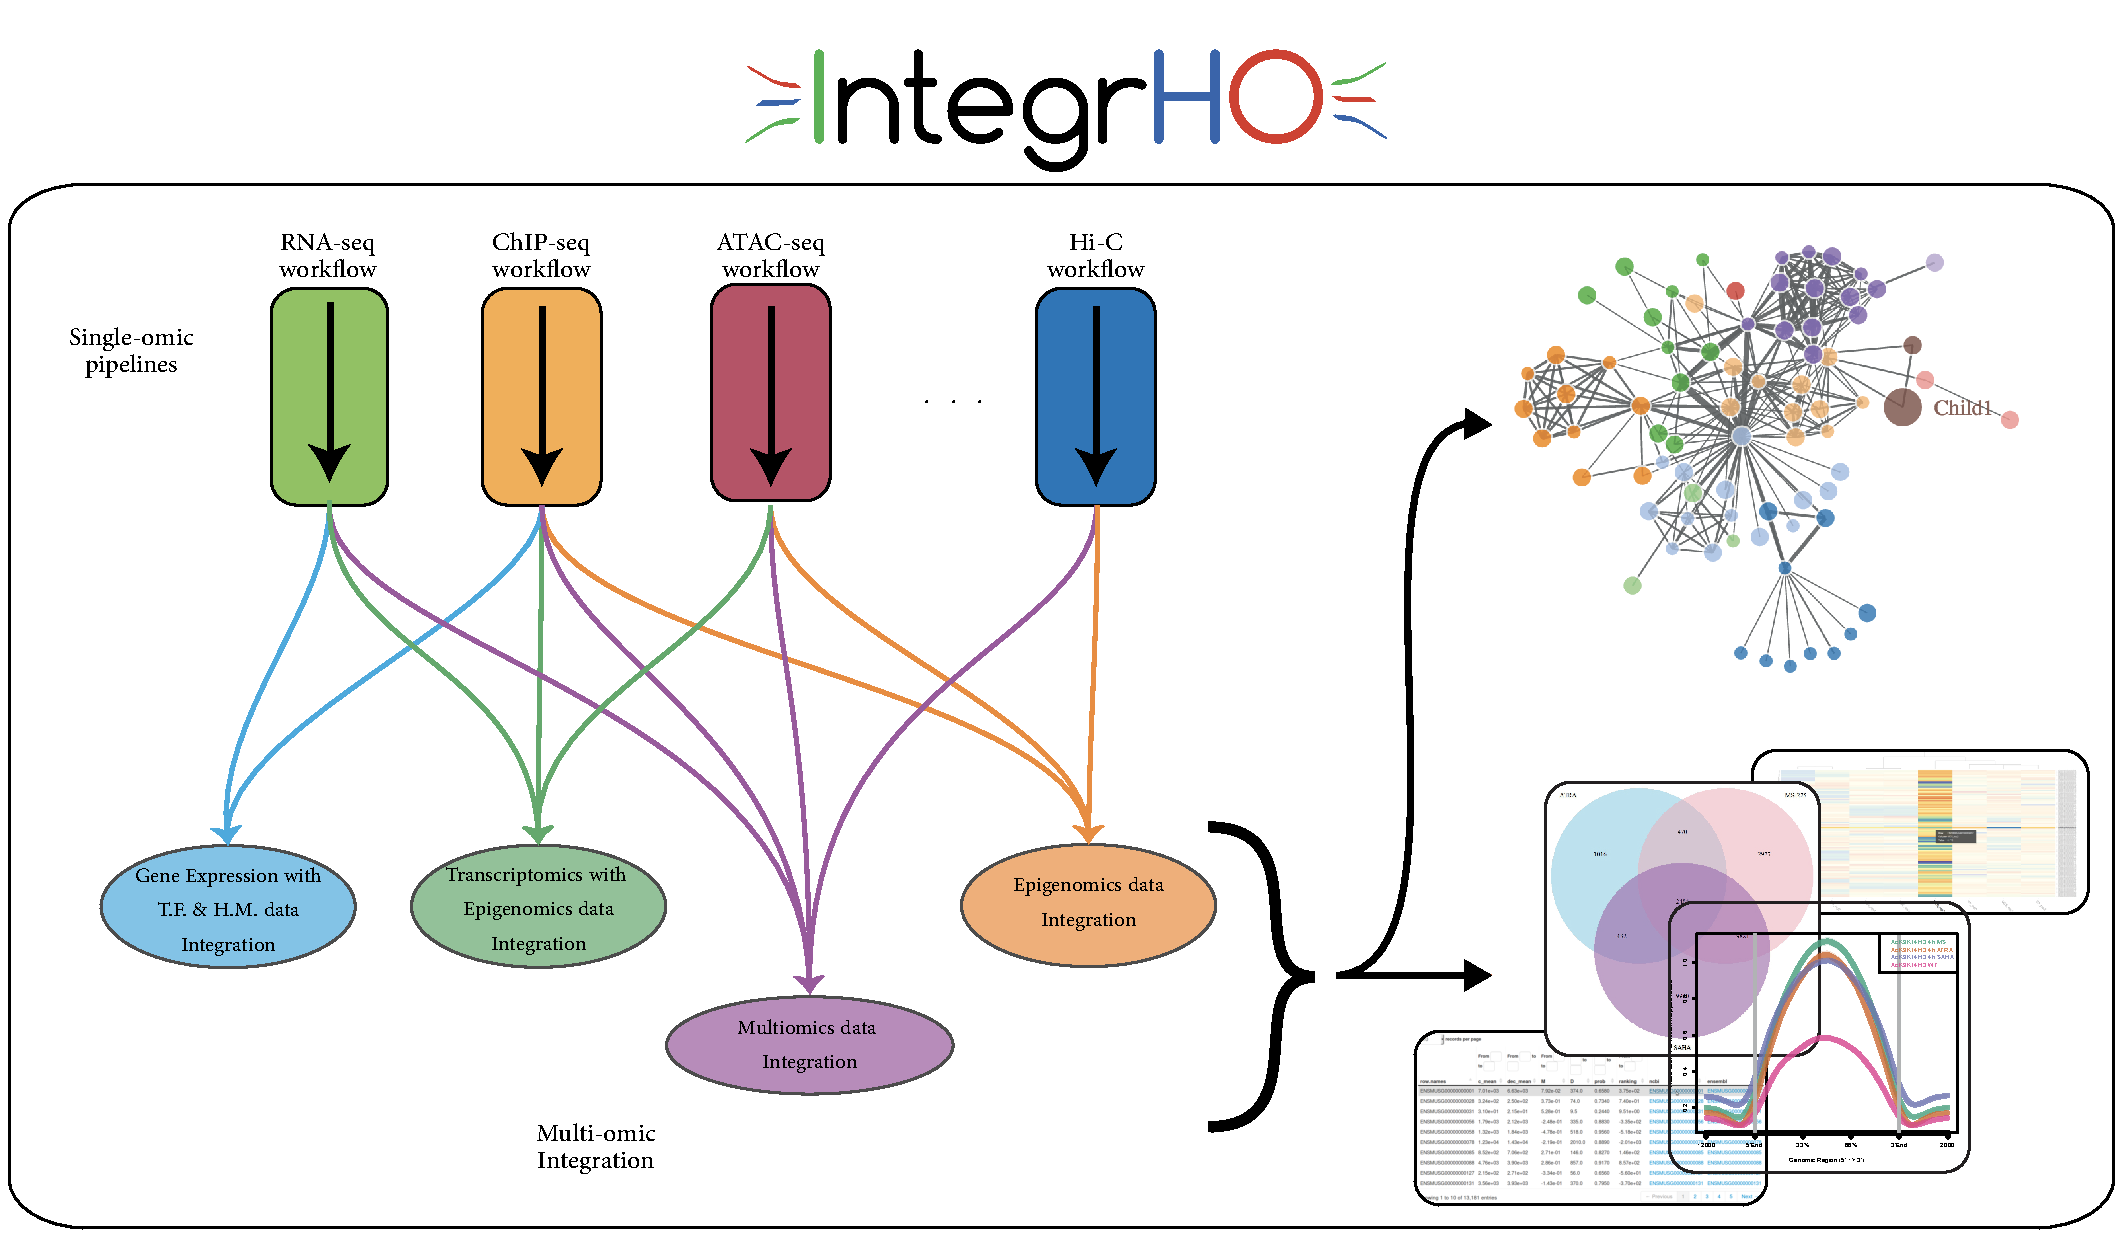
\includegraphics[width=\textwidth, keepaspectratio]{img/integrho/integrho_scheme.pdf}
\caption[integrho representation]{A schematical representation of \gls{igro} underlying idea.}
\label{fig:integrhoidea}
\end{figure}

For each -omics, \gls{igro} takes as input BAM or BED files, previously defined inside the design matrix of the main project definition interface.

Moreover, not only our software offers lots of utilities for data management and analysis, but also a great variability of graphics, useful to explore data and results, both in pre-processing and post-processing phase, such as \textit{barplots}, \textit{correlation plots}, \textit{heatmap}, \textit{scatterplots}, etc.

In order to facilitate the multi-omic data integration, we assembled several R functions to be freely combined in order to analyse each single-omic data type and to use their results for multi-omic data integration (Figure 1).

For \textit{RNA-seq} we constructed a dedicated interface for each step of a standard \textit{RNA-seq} data analysis pipeline, such as to build a count matrix, to filter out low counts with multiple tests, to normalize them and to account for batch effect.
Moreover, we selected multiple methods for \gls{deg}, such as \textit{edgeR}, \textit{DESeq2}, \textit{NOISeq}.

For \textit{ChIP-Seq} we constructed specific interfaces for peak calling, annotation and \glspl{der} detection.
For the peak calling, because of the lack of specific methods starting from BAM files, we implemented a dedicated interface for \textit{csaw}\cite{Lun2015} peak caller, which allows quantification for both broad and narrow peaks, typically resulting from \gls{hm} and \gls{tf} \textit{ChIP-seq} data.

For the annotation we selected the \textit{ChIPpeakAnno} and the \textit{ChIPseeker} R/Bioconductor packages, which produces similar output formats starting from peaks.
While for the detection of \glspl{der} we used the same methods as for \textit{RNA-seq}.

For \textit{ATAC-Seq} we used mostly the same methods implemented for the \textit{ChIP-Seq}, but designing specific interfaces for the filtering/alignment and the counting matrix as implemented in the \textit{DEScan2} package (see chapter \ref{sec:descan2cap} for further details).

To provide an integration of these -omics, we dedicated an entire section to this aspect, with functionalities for the annotation of \glspl{der} with \glspl{deg} using \textit{ChIPpeakAnno} and to use this information to investigate the functional response by enrichment for Gene Ontology or for Pathways.
These last two aspects implemented with aid of \textit{g:Profiler} \cite{Reimand2016} and \textit{graphite} \cite{Sales2012a} R/Bioconductor packages.


\section{TiCoRSe - Time Course RNA-Seq data analysis}
\input{sections/ticorsemethods.tex}

\section{DEScan2 - Differential Enriched Scan 2}
\input{sections/descanmethods.tex}

\section{IntegrHO - Integration of High-Throughtput Omics data}
\input{sections/integrhomethods.tex}

\chapter{Results}
\section{TiCoRSe - Time Course RNA-Seq data analysis}
\section{DEScan2 - Differential Enriched Scan 2}
\section{IntegrHO - Integration of High-Throughtput Omics data}

\chapter{Future Works}

\chapter{Conclusions}

\begin{appendices}
\include{appendixA}
%\include{appendixB}
%\include{appendixC}
\end{appendices}

%This chapter explains some basic information useful to understand the context where this thesis work has been developed.
Explaining some biological basic aspects and how it is possible to study the cellular behaviour from multiple points of view using different sequencing techniques.
%\include{aim_of_the_study}
%\include{MVDA}
%\include{INSIdEnano}
%\include{discussion}
%\include{conclusion}

%\begin{appendices}
%\include{appendixA}
%\include{appendixB}
%\include{appendixC}
%\end{appendices}

\printbibliography[heading=bibnumbered]

\cleardoublepage
% \phantomsection
\addcontentsline{toc}{chapter}{\listfigurename}
\listoffigures

\cleardoublepage
% \phantomsection
\addcontentsline{toc}{chapter}{\listtablename}
\listoftables

%\listoffigures
%\listoftables

\end{document}